\chapter{Neuronales Netz}
\label{ch:neuronalesNetz}
Im folgenden Kapitel wird das Training eines neuronalen Netzes eingeleitet und überwacht. Die dafür benötigten Testdaten 
werden strukturier, aufbereitet und anschließend zum Training vorbereitet und verwendet. Das trainierte Model soll für später
folgende Anwendungen aufrufbar sein um Vorhersagen in Echtzeit zu tätigen.

Sowohl über ein Webdienst als auch über ein Deployment soll das trainierte Model Verfügbar sein. Dafür werden, wie in 
Abbildung~\ref{fig:schematische_architektur} auf Seite~\pageref{fig:schematische_architektur} zu sehen, zwei unterschiedliche
Anwendungen angelegt und eingerichtet.

Die Kommunikation mit den Anwendungen geschieht über den Austausch von JSON-Objekten über REST-Schnittstellen. Damit die 
Kommunikation zentral gesteuert sowie einfach wartbar ist, soll ein API-Gateway zwischen Anwendung und den beiden Deployments
für komfort sorgen.  

Der API-Gateway-Service \textit{API Connect} verfügt über zwei verwaltete Endpunkte. Einer steht für die Kommunikation
mit dem Webdienst. Der Andere für die Kommunikation mit dem Deployment.

Ziel der Architektur ist die Bereitstellung eines trainierten Models, welches aus einem neuronalen Netz hervorgeht. Die 
Architektur soll so aufgebaut werden, dass sie im Weiteren gut Wartbar und Erweiterbar ist.

Außerdem soll ein Test ergeben, ob das selbe trainierte Model auch unter zwei verschiedenen Implementierungen zum gleichen 
Ergebnis für Vorhersagen mit den gleichen Eingabeparametern kommt und warum es eventuell Abweichungen geben kann.

\begin{figure}[h]
    \centering
    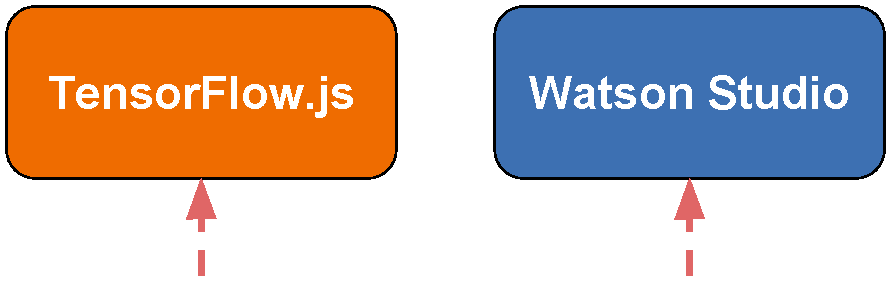
\includegraphics[scale=0.5]{images/kapitel_3/architektur_schematisch.pdf}
    \caption{Schematische Darstellung der Architektur}
    \label{fig:schematische_architektur}
\end{figure}